\section{Assembler}
\subsection{Interaction with Memory}
The CPU uses 32-bit sized instructions to
\begin{enumerate}[leftmargin=20pt]
    \item read memory (DRAM) into registers if needed
    \item execute computation using registers
    \item write the changed registers back into memory (DRAM)
\end{enumerate}

\newpar{}
\textbf{Remark:} While the CPU always uses 32-bit sized instructions to access memory, 
the address space can be larger:

\renewcommand{\arraystretch}{1.3}
\setlength\tabcolsep{6pt} % default value: 6pt
\begin{tabularx}{\linewidth}{@{}lll@{}}
    Name        & Register size & Address space          \\
    \cmidrule{1-3}
    \code{RV32} & 32 bit        & $2^{32} \simeq 4$ Gbit \\
    \code{RV64} & 64 bit        & $2^{64} \gg 1$ Pbit    \\
\end{tabularx}
\renewcommand{\arraystretch}{1}
\setlength\tabcolsep{6pt} % default value: 6pt

\subsection{Signedness}
$n$ bits can either represent [0,$2^{n}-1$] \textbf{unsigned} or [$-2^{n-1}, 2^{n-1}$] \textbf{signed} numbers.
For \textbf{signed} numbers the \textbf{two's complement}
\noindent\begin{equation*}
    -a_{n-1}\cdot2^{n-1}+\sum_{i=0}^{n-2}a_{i}\cdot 2^{i}
\end{equation*}
is used, which allows for addition and subtraction with only one command.

\subsection{Useful Instructions}
RISC-V instruction set architecture (isa) \code{RV32I} can be found in Section\ \ref{riscv_isa}.

\subsection{Big-/ Little-Endian}
A given register \code{t1 = [0xAA,0xBB]} can be represented in memory as

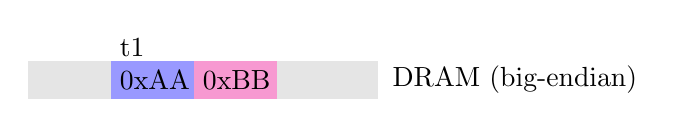
\begin{tikzpicture}

    \node[rectangle,
        text width = 30pt,
        text height = 7pt,
        draw = none,
        text = black,
        fill = gray!20] (r) at (0,0) {};

    \node[rectangle,
        text width = 30pt,
        text height = 7pt,
        draw=none,
        text = black,
        fill = blue!40] (r) at (30pt,0) {\fncode{0xAA}};

    \node[rectangle,
        text width = 30pt,
        text height = 7pt,
        draw=none,
        text = black,] at (30pt,12pt) {\fncode{t1}};

    \node[rectangle,
        text width = 30pt,
        text height = 7pt,
        draw=none,
        text = black,
        fill = magenta!40] (r) at (60pt,0) {\fncode{0xBB}};

    \node[rectangle,
        text width = 30pt,
        text height = 7pt,
        draw = none,
        text = black,
        fill = gray!20] (r) at (90pt,0) {};

    \node[rectangle,
        anchor = west,
        text height = 7pt,
        draw=none,
        text = black,] at (110pt,0pt) {\fncode{DRAM (big-endian)}};

\end{tikzpicture}

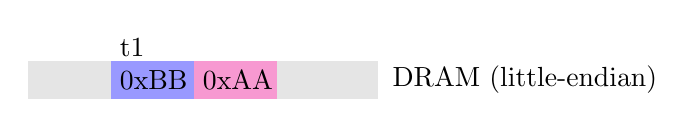
\begin{tikzpicture}

    \node[rectangle,
        text width = 30pt,
        text height = 7pt,
        draw = none,
        text = black,
        fill = gray!20] (r) at (0,0) {};

    \node[rectangle,
        text width = 30pt,
        text height = 7pt,
        draw=none,
        text = black,
        fill = blue!40] (r) at (30pt,0) {\fncode{0xBB}};

    \node[rectangle,
        text width = 30pt,
        text height = 7pt,
        draw=none,
        text = black,] at (30pt,12pt) {\fncode{t1}};

    \node[rectangle,
        text width = 30pt,
        text height = 7pt,
        draw=none,
        text = black,
        fill = magenta!40] (r) at (60pt,0) {\fncode{0xAA}};

    \node[rectangle,
        text width = 30pt,
        text height = 7pt,
        draw = none,
        text = black,
        fill = gray!20] (r) at (90pt,0) {};

    \node[rectangle,
        anchor = west,
        text height = 7pt,
        draw=none,
        text = black,] at (110pt,0pt) {\fncode{DRAM (little-endian)}};

\end{tikzpicture}

RISC-V uses little-endian.